%!TEX root = ../Thesis.tex
\section{Installation}
\label{instal}

\subsection{TeX-Distribution}

Für die Arbeit mit \LaTeX ist eine aktuelle TeX-Distribution erforderlich. 

\subsubsection{Windows}

Unter Windows ist MiKTeX die Standard-{\LaTeX}-Distribution. Der MikTex-Installer kann unter \url{http://miktex.org/download} heruntergeladen werden.

\subsubsection{Linux}

Die Standard-{\LaTeX}-Distribution unter Linux ist Tex Live, welche über die gängigen Software-Repositories installiert werden kann.

Unter Debian/Ubuntu kann die Installation der erforderlichen Pakete mittels der folgenden Befehlen durchgeführt werden:

\texttt{sudo apt-get install texlive-latex-base}\\
\texttt{sudo apt-get install texlive-latex-recommended}\\
\texttt{sudo apt-get install texlive-fonts-recommended}\\
\texttt{sudo apt-get install biblatex}\\
\texttt{sudo apt-get install biber}

\subsubsection{Mac-OS}
Von der Tex-User-Group wird jährlich ein komplettes aktuelles Mac{\TeX}-Paket angeboten (http://www.tug.org/mactex/index.html), in dem alle relevanten Programme und Pakete enthalten sind.

\subsection{PDF-Viewer}

\subsubsection{Windows}

Als PDF-Viewer unter Windows bietet sich der freie Sumatra PDF Viewer an: \url{http://blog.kowalczyk.info/software/sumatrapdf/download-free-pdf-viewer-de.html}

\subsubsection{Linux und Mac-OS}

Die installierten Standard-PDF-Viewer unter Linux bzw. Mac-OS können problemlos genutzt werden.

\subsection{Hello World}
Nach der Installation sollte ein erster Test der Vorlage versucht werden. Dazu öffnen Sie ein Kommandozeilenfenster und wechseln in das Verzeichnis, in dem sich die {\LaTeX}-Quellen dieser Vorlage befinden. Anschließend müssen auf der Kommandozeile die Befehle 
\begin{lstlisting}
  biber Thesis
  pdflatex Thesis
\end{lstlisting}
eingegeben werden. Nun sollte eine neue Datei \texttt{Thesis.pdf} erzeugt worden sein. Falls nicht, sehen Sie bitte in den Ausgaben nach, die \LaTeX erzeugt hat. Diese sind recht umfangreich, auch wenn ein PDF-Dokument erzeugt werden konnte.


\subsection{Literaturverwaltung}

Für die Verwaltung von Quellen eignet sich das freie, Cloud-basierte Mendely: \url{http://www.mendeley.com/download-mendeley-desktop/}. 

\begin{figure}[hbt]
\centering
\begin{minipage}[t]{1\textwidth} % Breite, z.B. 1\textwidth		
\caption{Mendeley Referenzmanager} % Überschrift
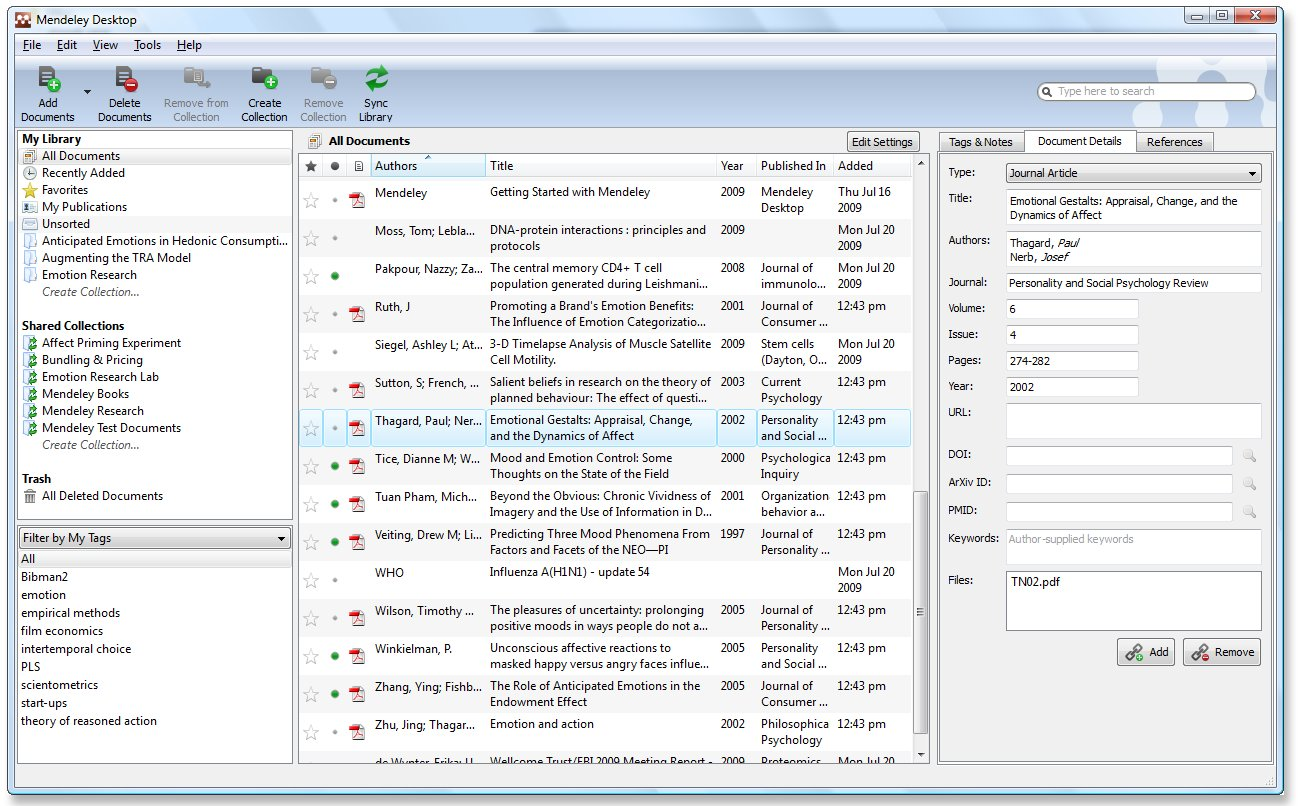
\includegraphics[width=1\textwidth]{img/Mendeley-destop-screenshot}\\ % Pfad
\source{\url{http://dominique-fleury.com/?p=302}} % Quelle
\end{minipage}
\end{figure}

\subsection{Texteditor}

Als Texteditor für \LaTeX wird Sublime Text (\url{http://www.sublimetext.com}) empfohlen. Zur Arbeit mit Latex ist das Plugin \emph{LaTeXTools} erforderlich (\url{https://github.com/SublimeText/LaTeXTools}).

\begin{figure}[hbt]
\centering
\begin{minipage}[t]{1\textwidth} % Breite, z.B. 1\textwidth		
\caption{Sublime Texteditor} % Überschrift
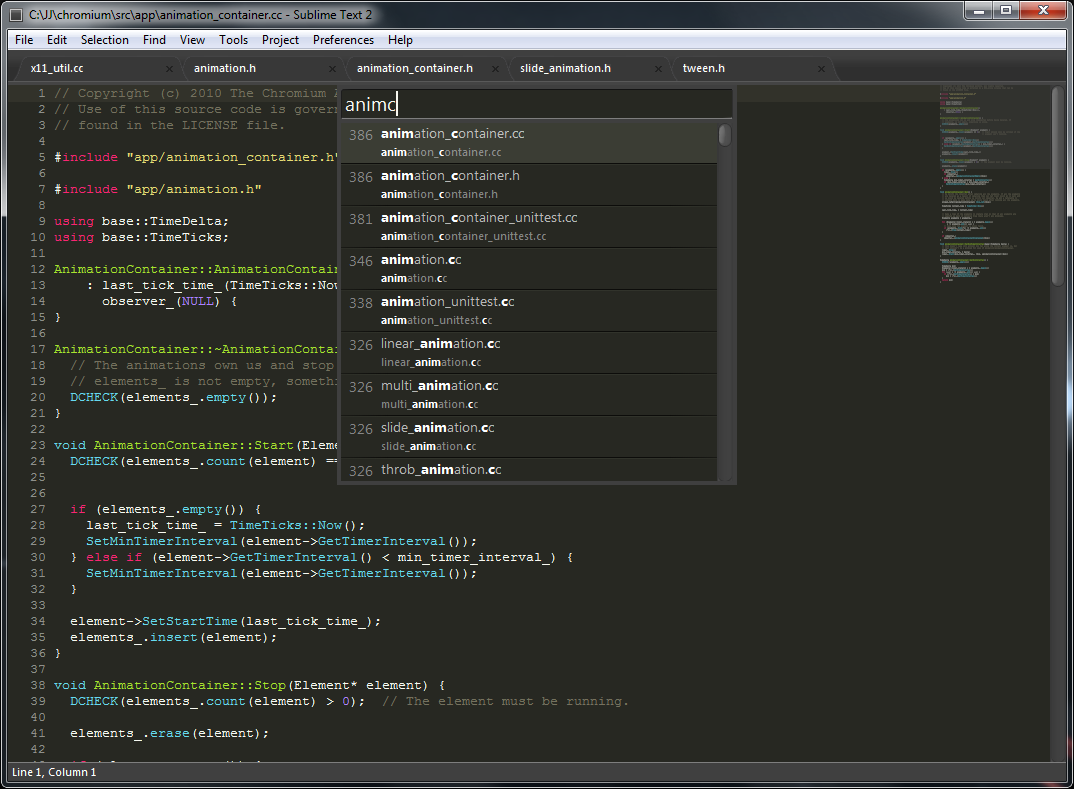
\includegraphics[width=1\textwidth]{img/sublime.png}\\ % Pfad
\source{\url{http://www.sublimetext.com/screenshots/alpha_goto_anything2_large.png}} % Quelle
\end{minipage}
\end{figure}

\subsection{PDF-Erzeugung}

Für die Erzeugung des PDF-Dokuments inklusive Referenzen, Quellenverzeichnis und Glossar sind mehrere Programmaufrufe und -durchläufe erforderlich. Der vollständige Aufruf zur PDF-Erzeugung lautet: 

\texttt{pdflatex Thesis}\\
\texttt{biber Thesis}\\
\texttt{makeindex -s Thesis.ist -t Thesis.alg -o Thesis.acr Thesis.acn}\\
\texttt{makeglossaries Thesis}\\
\texttt{pdflatex Thesis}\\
\texttt{pdflatex Thesis}\\